\documentclass[12pt, a4paper]{article}

\title{Dipole emission near a planar multilayer stack}
\author{Baptiste Augui\'e}    
\date{\today}
\usepackage{siunitx}
\usepackage{amsmath,amssymb}% AMS standards    
\usepackage[utf8]{inputenc}

% \VignetteIndexEntry{planar}
\bibliographystyle{alpha}

\usepackage{/Library/Frameworks/R.framework/Resources/share/texmf/tex/latex/Sweave}
\begin{document}

\setkeys{Gin}{width=\textwidth}

\newcommand{\dq}{\text{d}q} 
\newcommand{\du}{\text{d}u} 

\maketitle
\begin{abstract}
The \texttt{planar} package solves the electromagnetic problem of dipole emission near a planar multilayer stack. It comprises two sets of functions; i) to compute the effective Fresnel reflection coefficient of a multilayer structure; ii) to evaluate the modified dipolar field as an integral over plane waves reflected at the interface.
\end{abstract}



\section{Fresnel coefficients}

The functions \texttt{recursive.fresnel} and \texttt{multilayer} both
compute the Fresnel coefficients for a multilayer stack, using two
different methods (recursive application of Fresnel coefficients for a
layer; and transfer matrix, respectively). \texttt{multilayer} is more versatile in that it also returns the fields and enhancement factors. \texttt{recursive.fresnel},  on the other hand, is more robust for some calculations involving lossless layers. Both functions are complemented by a faster implementation in \texttt{C++}, though the output is not as comprehensive.
%
\subsection{Multilayer optics}
%
\begin{figure}[!ht]
\centering
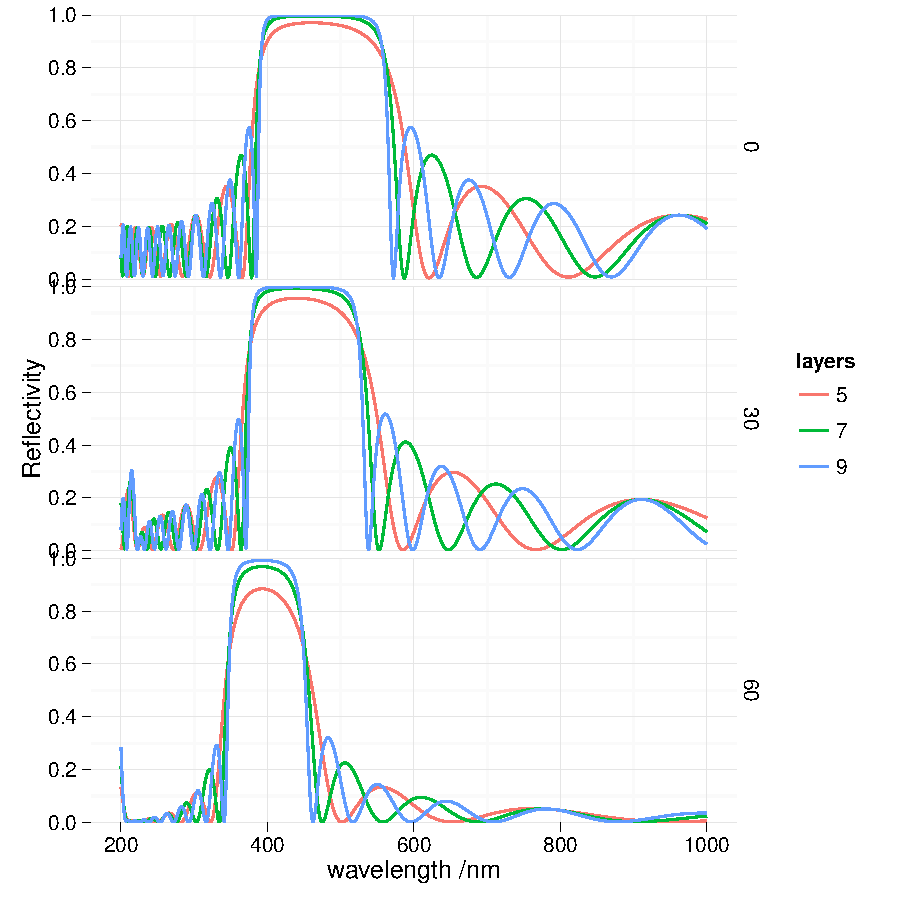
\includegraphics{planar-vignette-bragg_stack}
\caption{\texttt{demo(bragg\_stack)}. Reflectivity of a Bragg stack with varying number of layers. Reproducing Fig. 6.6, p. 188 of Mac Leod's Thin Film Optical Filters the structure is a stack of lambda/4 layers of indices nH and nL on a glass substrate with increasing number of layers, the reflectivity stop-band becomes stronger.}
\label{fig:braggstack}
\end{figure}

\begin{figure}[!ht]
\centering
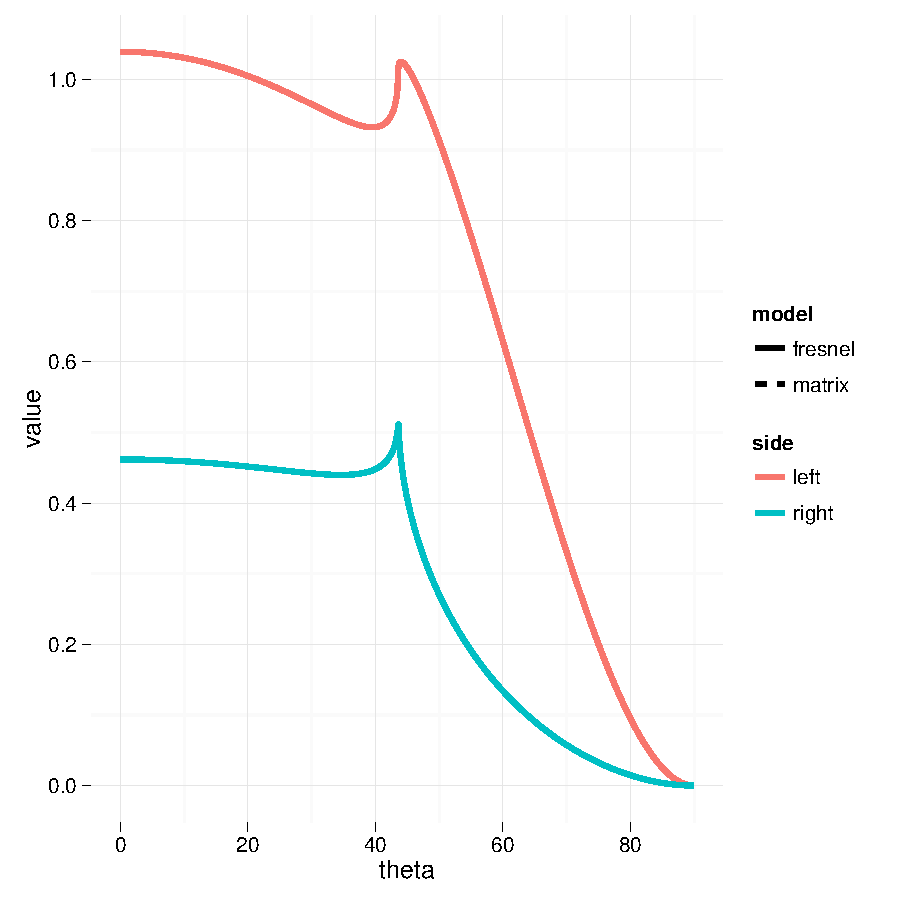
\includegraphics{planar-vignette-field_enhancement}
\caption{\texttt{demo(LFIEF\_distance)}. Comparison of the near field enhancement outside of a thin metal film, calculated with i) the transfer matrix method of \texttt{multilayer}; ii) Fresnel reflection and transmission coefficients.}
\label{fig:fieldenhancement}
\end{figure}

